A power analysis was successful for all contrasts.  Results of the estimation procedure for the prevalence of activation $\pi_1$ and the effect size based on a pilot dataset of about 15 subjects are shown in Figure \ref{HCP_pi1}.  We show that for a range of contrasts and tasks we find overestimated estimates for the prevalence of activation.  The estimations are good with low variance and the effect sizes suffer from modest overestimation.  For the effect sizes, we find - as in the simulations - underestimation for smaller (more local) effect sizes.

\begin{center}
\begin{figure}[h]
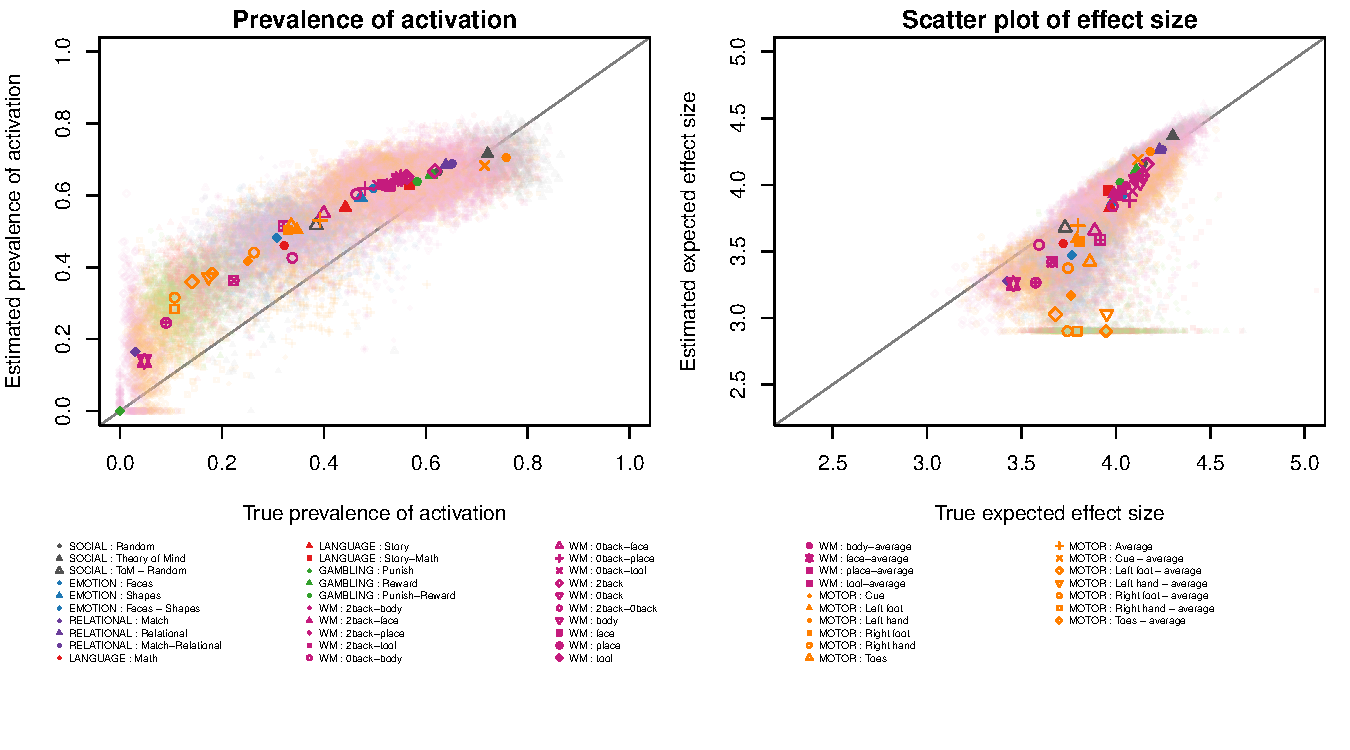
\includegraphics[scale=0.8]{FIG_HCP_15_modelestimation.pdf}
\caption{An evaluation of the estimation of $\pi_1$ (left) and the effect size (right).  Each pastel colored plotting symbol corresponds to one random sub-sample taken from the data, for one particular sample size, experiment and contrast.  The average estimation for each contrast is plotted in a darker color. \label{HCP_pi1}}
\end{figure}
\end{center}

The estimation and bias on the power estimates for error rate control at 5\% is given in Figure \ref{HCP_bias}.  In most contrasts, the bias ranges from 10\% underestimation (blue) to 10\% overestimation (red).  In general, the underestimation occurs for lower values of power and disappears over a short range of subjects.  The underestimation is much larger for contrasts with a smaller effect size.
For larger values of power, the estimates are overestimated.  With power analysis methods assuming a parametric distribution, there will always be a point where 100 percent power is achieved.  However, in our estimation of the true power and the correction mechanism we apply, 100 percent power is never achieved.  Whether this is a true effect or an artifact of the mechanism is unfortunately unknown.
%As in the simulations, the adaptive multiple testing procedures show instability due to instances when no significant results are found, leading to underestimation of power.

%Again, the gambling task contrast, ``punish versus reward'', is problematic {\color{red} check if this is still the case}.  There are no resample schemes where both the pilot study resamples and the final study resamples result in the detection of active peaks.  As there is no activation, there is no finite solution for the average power defined in equation \ref{average power}.  %The same problem arises for some contrasts when thresholding with false discovery rate control.  As in the simulations, due to the adaptive character of the procedure, sometimes no significant effects are found.  This leads to infinite computations for power.

\begin{center}
\begin{figure}[h]
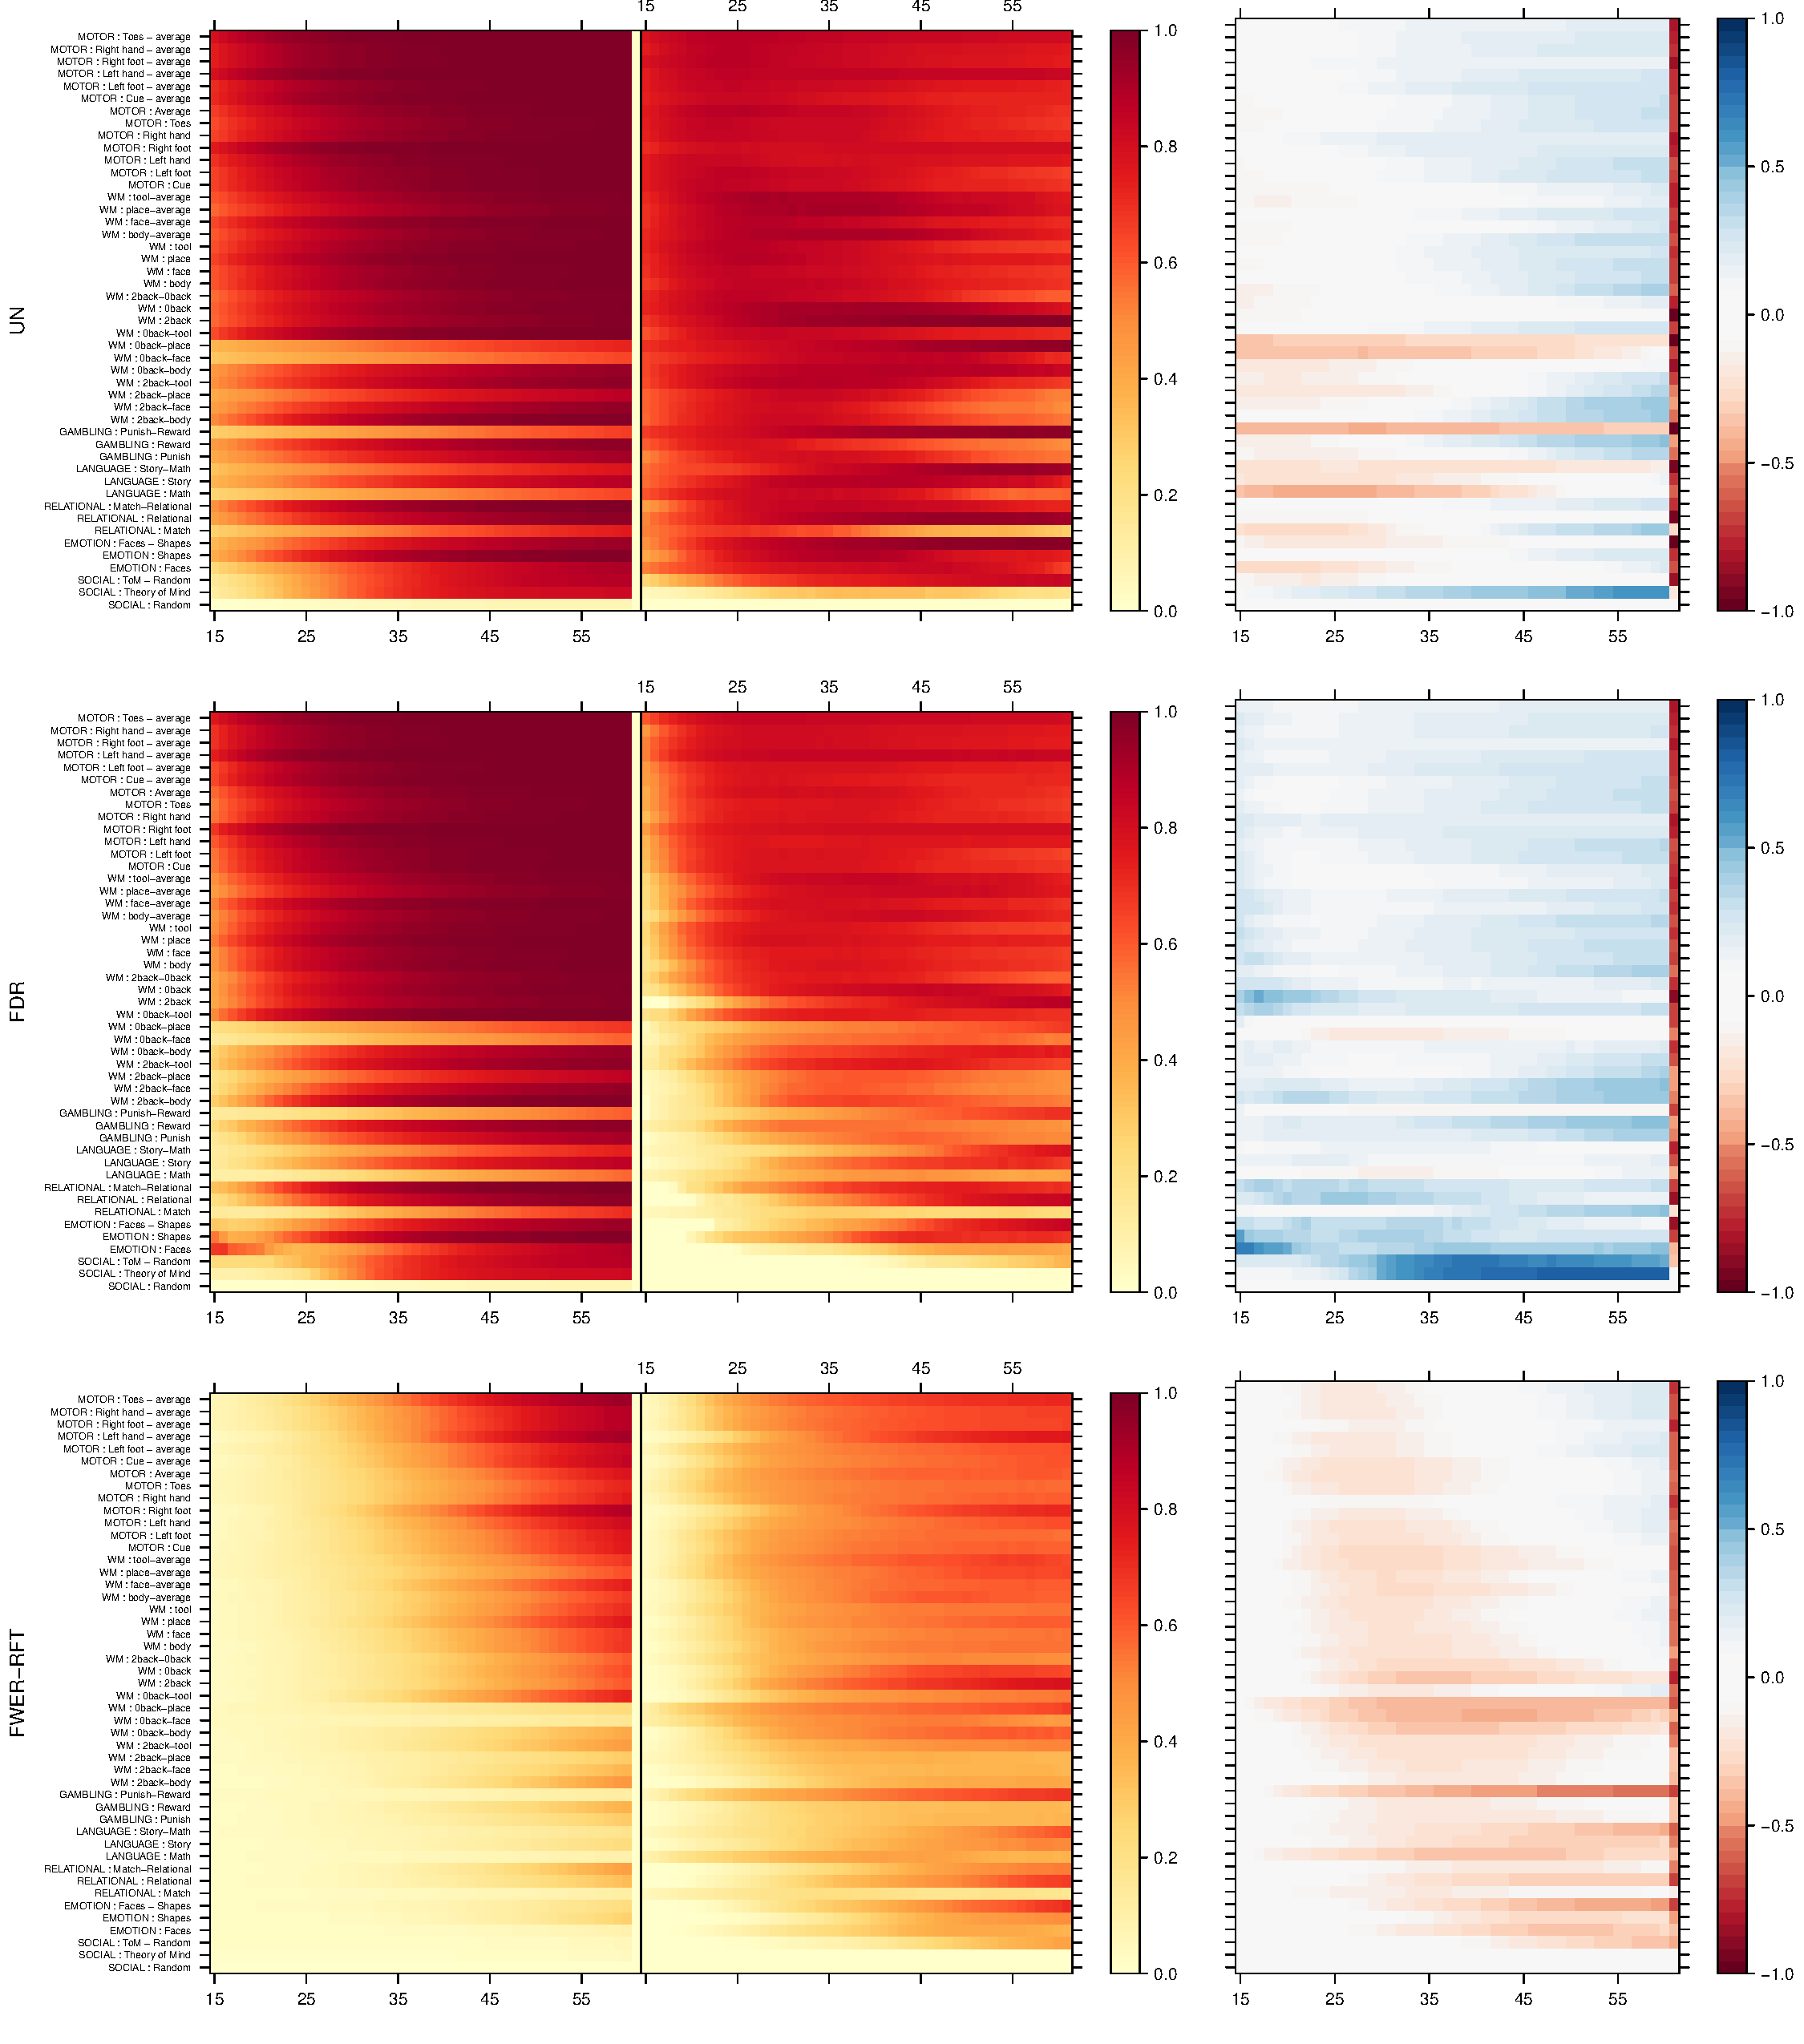
\includegraphics[scale=0.4]{FIG_HCP_15_power.pdf}
\caption{Evaluation of the power estimation over different subjects for all unique HCP-contrasts for thresholding with different error rate corrections at $\alpha=0.05$ from a pilot study with 15 subjects. The left column shows the estimated power curves, the middle column shows the true power and the right column shows the bias.  Bias is defined as the estimated power minus the true power.  The contrasts are sorted by their average empirically derived effect size. \label{HCP_bias}}
\end{figure}
\end{center}

Figure \ref{HCP_ss} shows the performance of the model when predicting sample sizes.  We see that over all contrasts, we see underestimation for thresholding using false discovery rate.  This result can be explained by the underestimation of our calculation of the threshold for the false discovery rate. % {\color{red} Add this to explanation of FDR}.
The motor contrasts show a larger overestimation of power with uncorrected thresholding.  This can be due to the fact that the motor contrasts are known to be very local contrasts. This corresponds to the results from the simulated condition when the percentage of active brain regions is small.

\begin{center}
\begin{figure}[h]
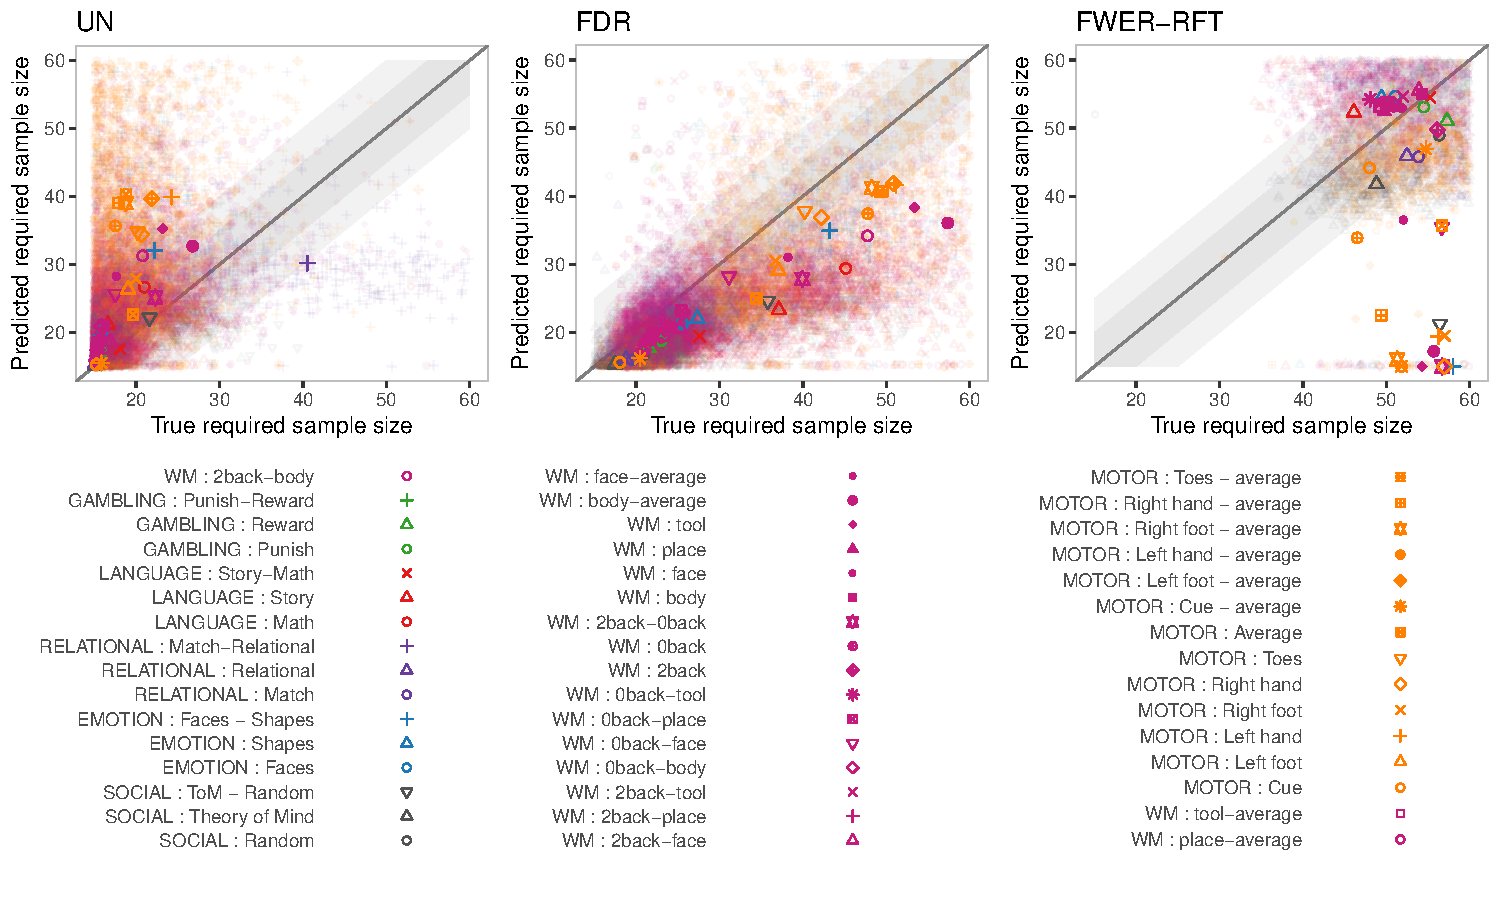
\includegraphics[scale=0.6]{FIG_HCP_15_sscalc.pdf}
\caption{Plots of the predicted and true required sample size when aiming for 80\% power. The different plots refer to the different multiple testing procedures.  Points inside the light grey area identify poins with a maximum bias of 15 subjects, the darker grey area refers to a maximum bias of 5 subjects.  Each semi-transparent dot represents a different subsample, as such there are 500 dots for each condition.  The fully colored dots present the average per task.  The estimated sample size results from a pilot study with 15 subjects. \label{HCP_ss}}
\end{figure}
\end{center}
